\documentclass[11pt]{beamer}

%%%%%%%%%%%%%%%%
% Packages
%%%%%%%%%%%%%%%%
\usepackage{booktabs}
\usepackage{hyperref}		% produces hyperlinks
\usepackage{multirow}	% allows for rows that span multiple rows in tables
\usepackage{multicol}
%%%%%%%%%%%%%%%%
% Prelims
%%%%%%%%%%%%%%%%

\usetheme[titleformat=smallcaps, progressbar=frametitle, block = fill]{metropolis}
\author{Sergio I. Garcia-Rios}
\title{Data colection + }
\institute{Government 3990: Statistics in the Social Science}
\date{}

%%%%%%%%%%%%%%%%%%%%%%%
% Style
%%%%%%%%%%%%%%%%%%%%%%%%5


%\setbeamertemplate{section in toc}{\inserttocsectionnumber.~\inserttocsection}
%\setbeamertemplate{subsection in toc}{$\qquad$\inserttocsubsectionnumber.~\inserttocsubsection \\}
%
%\AtBeginSection[] 
%{ 
%  \addtocounter{framenumber}{-1} 
%  % 
%  {\removepagenumbers 
%  {\small
%    \begin{frame}<beamer> 
%    \frametitle{Outline} 
%    \tableofcontents[currentsection] 
%  \end{frame} 
%  } 
%  }
%} 
%
%\AtBeginSubsection[] 
%{ 
%  \addtocounter{framenumber}{-1} 
%  % 
%  {\removepagenumbers 
%  {\small
%    \begin{frame}<beamer> 
%    \frametitle{Outline} 
%    \tableofcontents[currentsection,currentsubsection] 
%  \end{frame} 
%  } 
%  }
%}
%
%
%%%%%%%%%%%%%%%%%%5

% twocol: two columns
\newenvironment{twocol}[4]{
\begin{columns}[c]
\column{#1\textwidth}
#3
\column{#2\textwidth}
#4
\end{columns}
}

% threecol: three columns
\newenvironment{threecol}[6]{
\begin{columns}[c]
\column{#1\textwidth}
#4
\column{#2\textwidth}
#5
\column{#3\textwidth}
#6
\end{columns}
}


% solution stuff
\newcommand{\textitMult}[1]{
\only<1>{#1}
\only<2->{\alert{\textbf{#1}}}
}


\begin{document}
\maketitle

\begin{frame}[standout]
\Large{Data Collection + Observational studies \\ and experiments}
\end{frame}


\section{Use a sample to make inferences about the population}
\label{mi1}

%%%%%%%%%%%%%%%%%%%%%%%%%%%%%%%%%%%

\begin{frame}{1. Use a sample to make inferences about the population}
\small{
\begin{itemize}[<+->]
\item Ultimate goal: make inferences about populations
\item Caveat: populations are difficult or impossible to access
\item Solution: use a sample from that population, and use\alert{statistics} from that 
sample to make inferences about the unknown population \alert{parameters}
\item The better (more \alert{representative}) sample we have, the more reliable our 
estimates and more accurate our inferences will be



\item[] \footnotesize{
\begin{exampleblock}{Your Turn}
Suppose we want to know how many offspring female lemurs have, on average.
It's not feasible to obtain offspring data from on all female lemurs, so we use 
data from the Cornell Lemur Center. We use the sample mean from these data as an 
estimate for the unknown population mean. Can you see any limitations to using data 
from the Cornell Lemur Center to make inferences about all lemurs?
\end{exampleblock}
}

\end{itemize}
}
\end{frame}

%%%%%%%%%%%%%%%%%%%%%%%%%%%%%%%%%%%

\begin{frame}
\frametitle{Sampling is natural}

\begin{center}
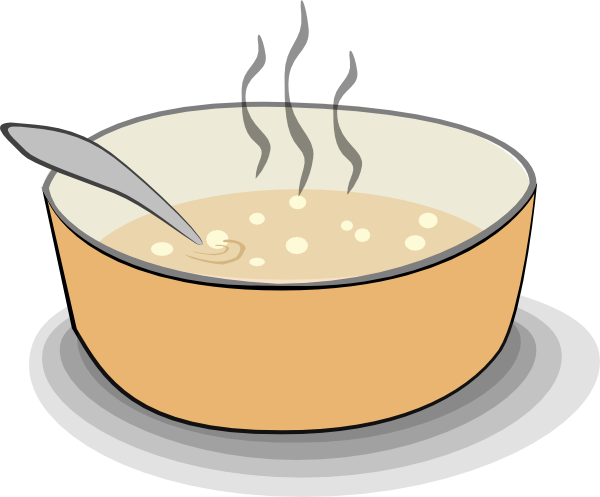
\includegraphics[width=0.3\textwidth]{figures/soup}
\end{center}

\begin{itemize}

\item When you taste a spoonful of soup and decide the spoonful you tasted isn't salty 
enough, that's \alert{exploratory analysis}

\item If you generalize and conclude that your entire soup needs salt, that's an \alert{
inference}

\item For your inference to be valid, the spoonful you tasted (the sample) needs to be 
\alert{representative} of the entire pot (the population)

\end{itemize}

\end{frame}

%%%%%%%%%%%%%%%%%%%%%%%%%%%%%%%%%%%

\section{Ideally use a simple random sample, stratify to control for a variable, and cluster to make sampling easier} 
\label{mi2}

%%%%%%%%%%%%%%%%%%%%%%%%%%%%%%%%%%%
\begin{frame}


\twocol{0.505}{0.51}{
\alert{Simple random:} \\
{\small Drawing names from a hat}
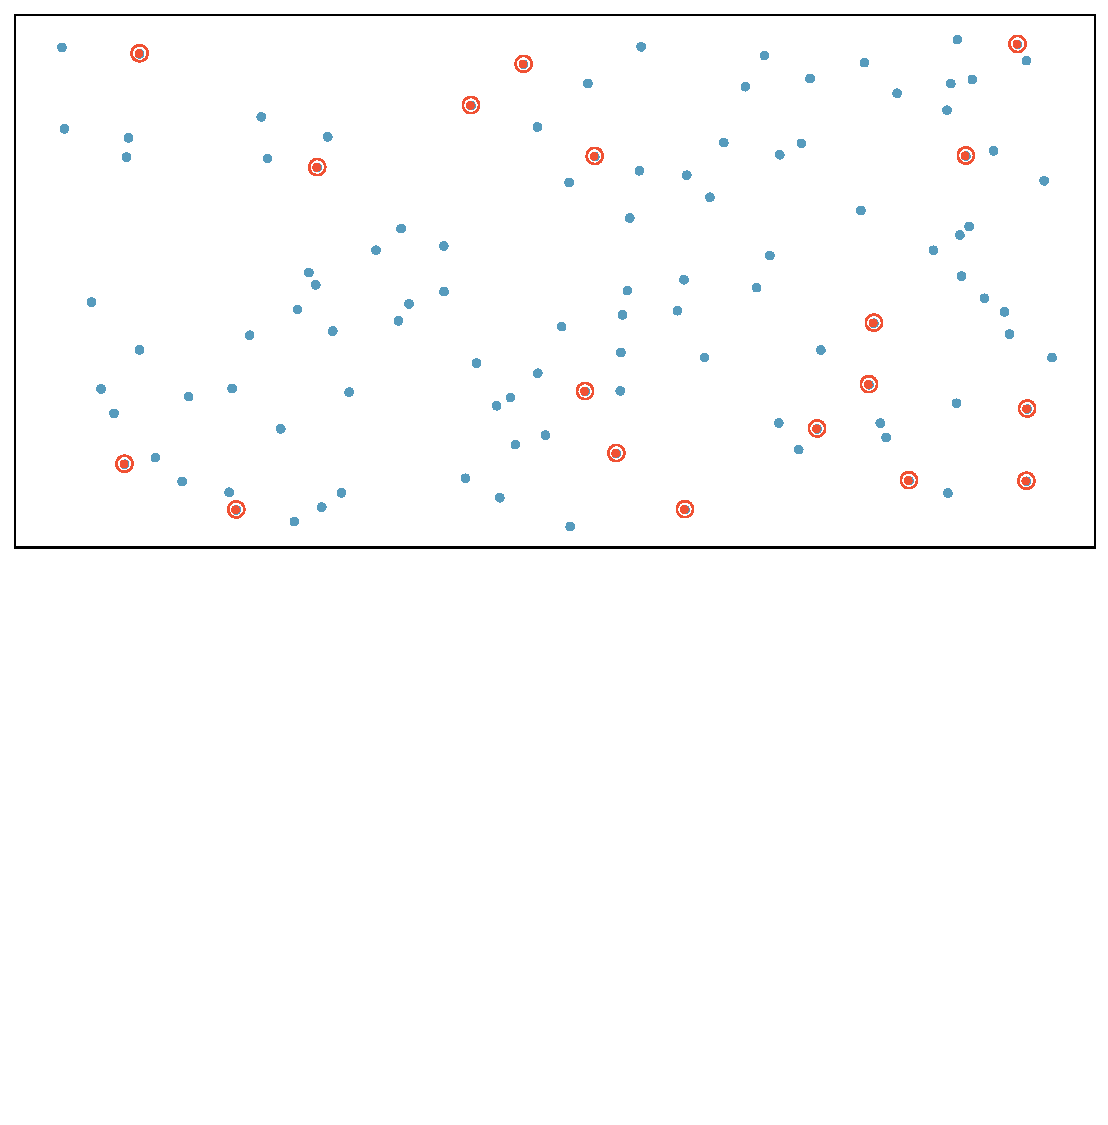
\includegraphics[width=\textwidth]{figures/sampling_simple} \\
\pause
\alert{Stratified:} {\small homogenous strata} \\
{\small Stratify to control for SES} \\
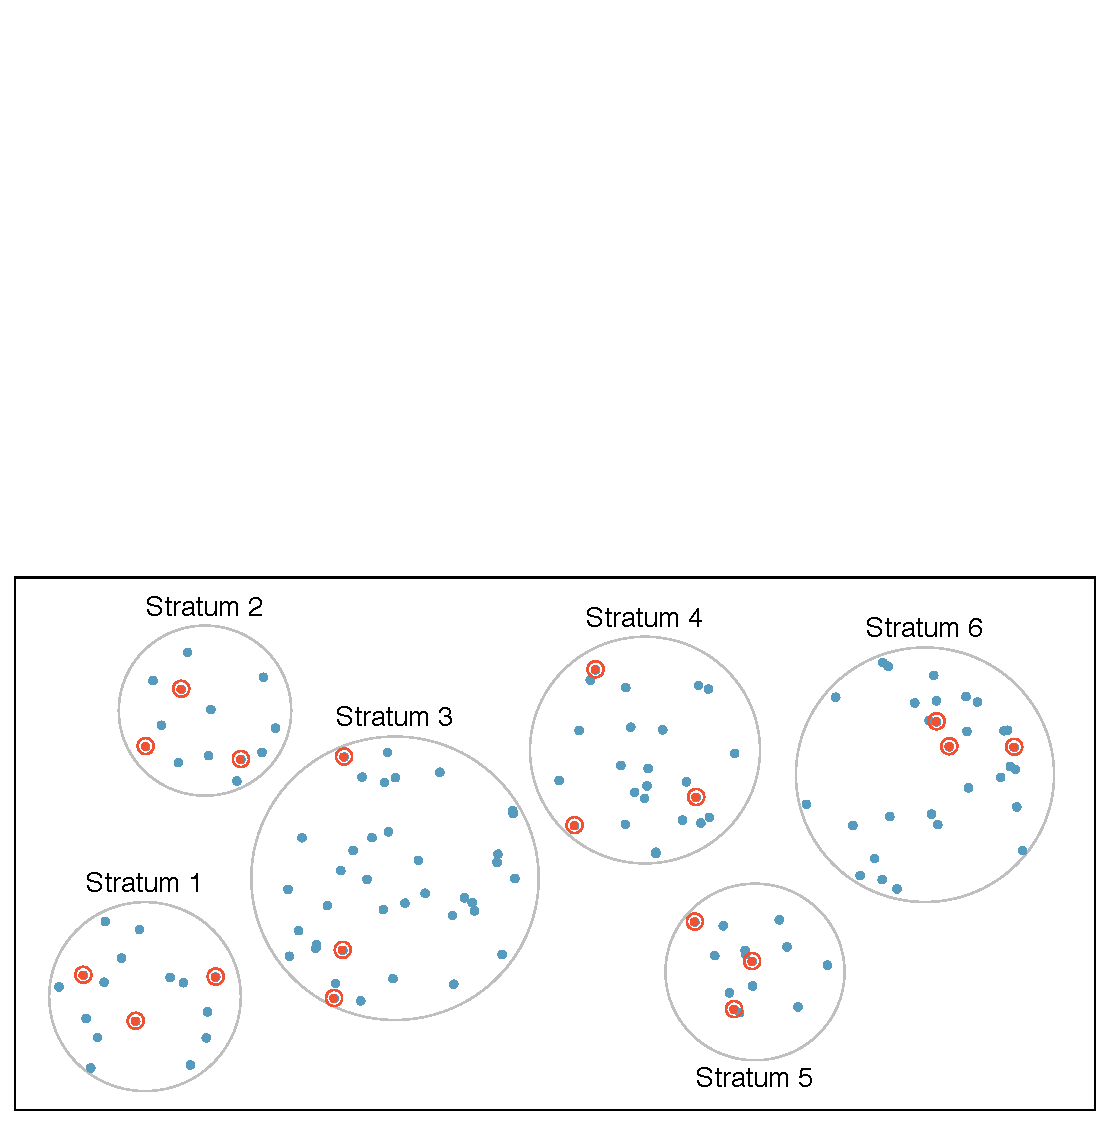
\includegraphics[width=\textwidth]{figures/sampling_stratified} 
}
{
\pause
\alert{Cluster:} {\small heterogenous clusters} \\
{\small Sample all chosen clusters}
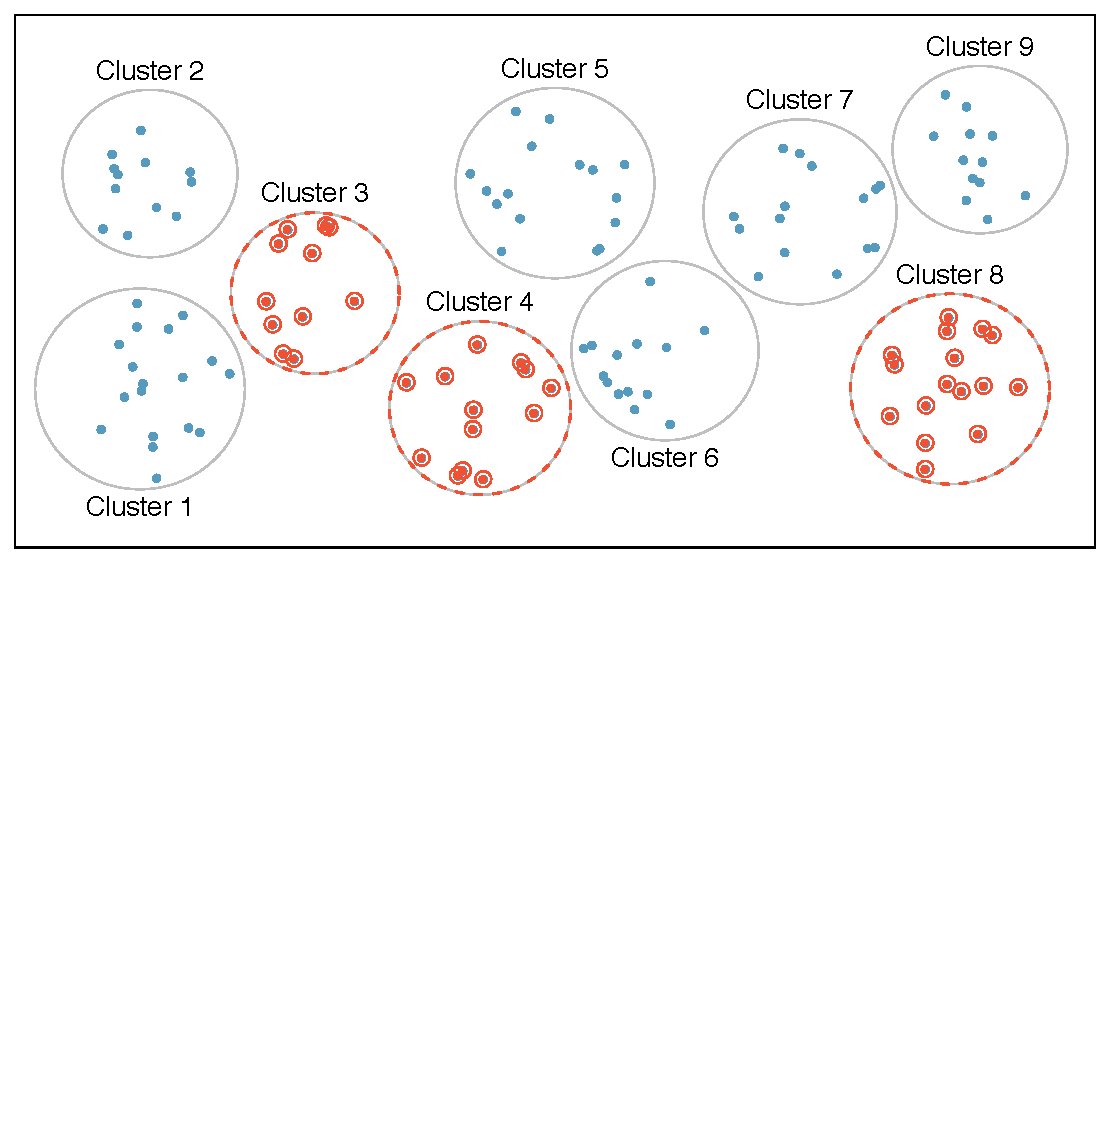
\includegraphics[width=\textwidth]{figures/sampling_cluster} \\
\pause
\alert{Multistage:} \\
{\small Random sample in chosen clusters}
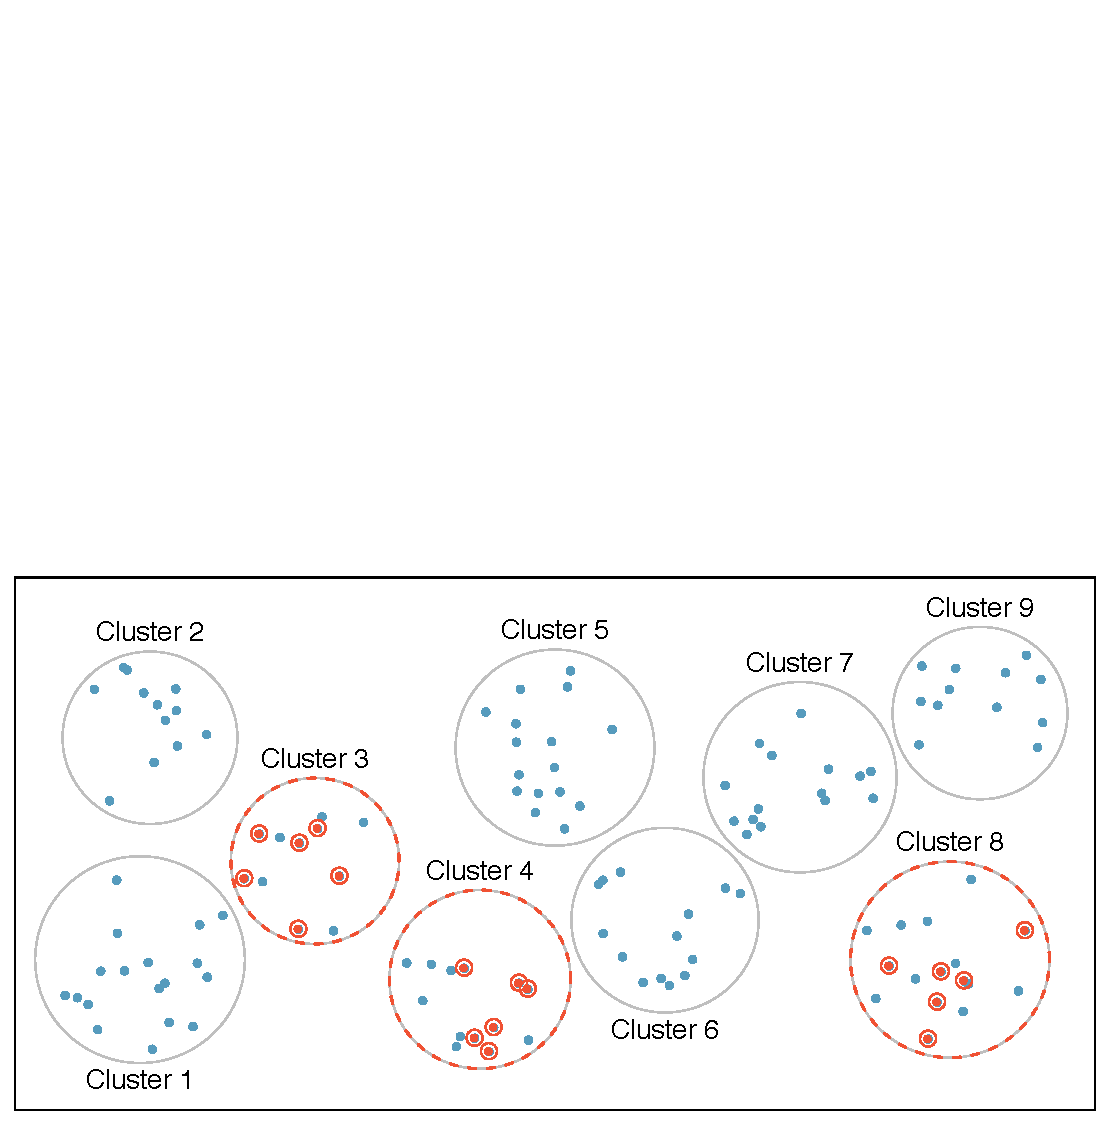
\includegraphics[width=\textwidth]{figures/sampling_multistage}
}

\end{frame}

%%%%%%%%%%%%%%%%%%%%%%%%%%%%%%%%%%%

\begin{frame}
\footnotesize{
\begin{exampleblock}{Your Turn}
A city council has requested a household survey be conducted in a suburban 
area of their city. The area is broken into many distinct and unique neighborhoods, 
some including large homes, some with only apartments, and others a diverse mixture of 
housing structures. Which approach would likely be the \emph{least} effective?\end{exampleblock}}

\begin{enumerate}[(a)]
\item Simple random sampling
\item Stratified sampling, where each stratum is a neighborhood
\item \textitMult{Cluster sampling, where each cluster is a neighborhood}
\end{enumerate}

\end{frame}

%%%%%%%%%%%%%%%%%%%%%%%%%%%%%%%%%%%

\section{Sampling schemes can suffer from a variety of biases}
\label{mi3}

%%%%%%%%%%%%%%%%%%%%%%%%%%%%%%%%%%%

\begin{frame}
\frametitle{3. Sampling schemes can suffer from a variety of biases}

\begin{itemize}[<+->]

\item \alert{Non-response:} If only a small fraction of the randomly sampled people choose 
to respond to a survey, the sample may no longer be representative of the population

\item \alert{Voluntary response:} Occurs when the sample consists of people who volunteer 
to respond because they have strong opinions on the issue since such a sample will also 
not be representative of the population

\item \alert{Convenience sample:} Individuals who are easily accessible are more likely to 
be included in the sample

\end{itemize}

\end{frame}

%%%%%%%%%%%%%%%%%%%%%%%%%%%%%%%%%%%

\begin{frame}[shrink]

{\small
\footnotesize{
\begin{exampleblock}{Your Turn}
A school district is considering whether it will no longer allow high school 
students to park at school after two recent accidents where students were severely 
injured. As a first step, they survey parents by mail, asking them whether or not the 
parents would object to this policy change. Of 6,000 surveys that go out, 1,200 are 
returned. Of these 1,200 surveys that were completed, 960 agreed with the policy change 
and 240 disagreed. Which of the following statements are true?
\end{exampleblock}}

\begin{enumerate}[I.]
\item Some of the mailings may have never reached the parents.
\item Overall, the school district has strong support from parents to move forward with 
the policy approval.
\item It is possible that majority of the parents of high school students disagree with 
the policy change.
\item The survey results are unlikely to be biased because all parents were mailed a 
survey. 
\end{enumerate}

\begin{multicols}{5}
\begin{enumerate}[(a)]
\item Only I
\item I and II
\item \textitMult{I and III}
\item III and IV
\item Only IV
\end{enumerate}
\end{multicols}
}

\end{frame}

%%%%%%%%%%%%%%%%%%%%%%%%%%%%%%%%%%%%

\section{Experiments use random assignment to treatment groups, observational studies do not}
\label{mi4}

%%%%%%%%%%%%%%%%%%%%%%%%%%%%%%%%%%%%

\begin{frame}

\begin{exampleblock}{}
What type of study is this? What is the scope of inference (causality / generalizability)?\footnote{http://www.nytimes.com/2014/06/30/technology/facebook-tinkers-with-users-emotions-in-news-feed-experiment-stirring-outcry.html}
\end{exampleblock}
\begin{center}
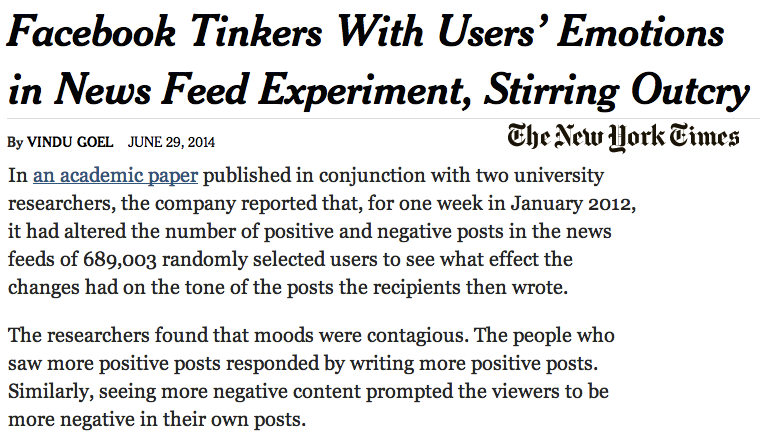
\includegraphics[width=0.9\textwidth]{figures/facebook_study}
\end{center}
%\scriptsize{
%\alert{\url{http://www.nytimes.com/2014/06/30/technology/facebook-tinkers-with-users-emotions-in-news-feed-experiment-stirring-outcry.html}}}

\end{frame}

%%%%%%%%%%%%%%%%%%%%%%%%%%%%%%%%%%%%%

\begin{frame}
\frametitle{4. Experiments use random assignment to treatment groups, observational studies do not}

{\small
\begin{exampleblock}{Your Turn}A study that surveyed a random sample of otherwise healthy adults found that people are more likely to get muscle cramps when they're stressed. The study also noted that people drink more coffee and sleep less when they're stressed. What type of study is this?
\end{exampleblock}

\textit{\onslide<2->{Observational}}

\begin{exampleblock}{What is the conclusion of the study?}\end{exampleblock}

\textit{\onslide<3->{There is an \alert{association} between increased stress \& muscle cramps.}}

\begin{exampleblock}{Can this study be used to conclude a causal relationship between increased stress and muscle cramps?}\end{exampleblock}

\textit{\onslide<4->{Muscle cramps might also be due to increased caffeine consumption or sleeping less -- these are potential \alert{confounding} variables.}}
}

\end{frame}

%%%%%%%%%%%%%%%%%%%%%%%%%%%%%%%%%%%%

\section{Four principles of experimental design: randomize, control, block, replicate}
\label{mi5}

%%%%%%%%%%%%%%%%%%%%%%%%%%%%%%%%%%%%

\begin{frame}
\frametitle{5. Four principles of experimental design:\\ randomize, control, block, 
replicate}

\begin{itemize}
\item We would like to design an experiment to investigate if increased stress causes 
muscle cramps:

\pause

\begin{itemize}
\item Treatment: increased stress
\item Control: no or baseline stress
\end{itemize}

\pause

\item It is suspected that the effect of stress might be different on younger and older 
people: \alert{block} for age.

\end{itemize}

\pause

\begin{alertblock}{Why is this important? Can you think of other variables to block for?}\end{alertblock}

\end{frame}

%%%%%%%%%%%%%%%%%%%%%%%%%%%%%%%%%%%

\section{Random sampling helps generalizability, random assignment helps causality}
\label{mi6}

%%%%%%%%%%%%%%%%%%%%%%%%%%%%%%%%%%%%

\begin{frame}
\frametitle{6. Random sampling helps generalizability,\\ random assignment helps 
causality}

\begin{center}
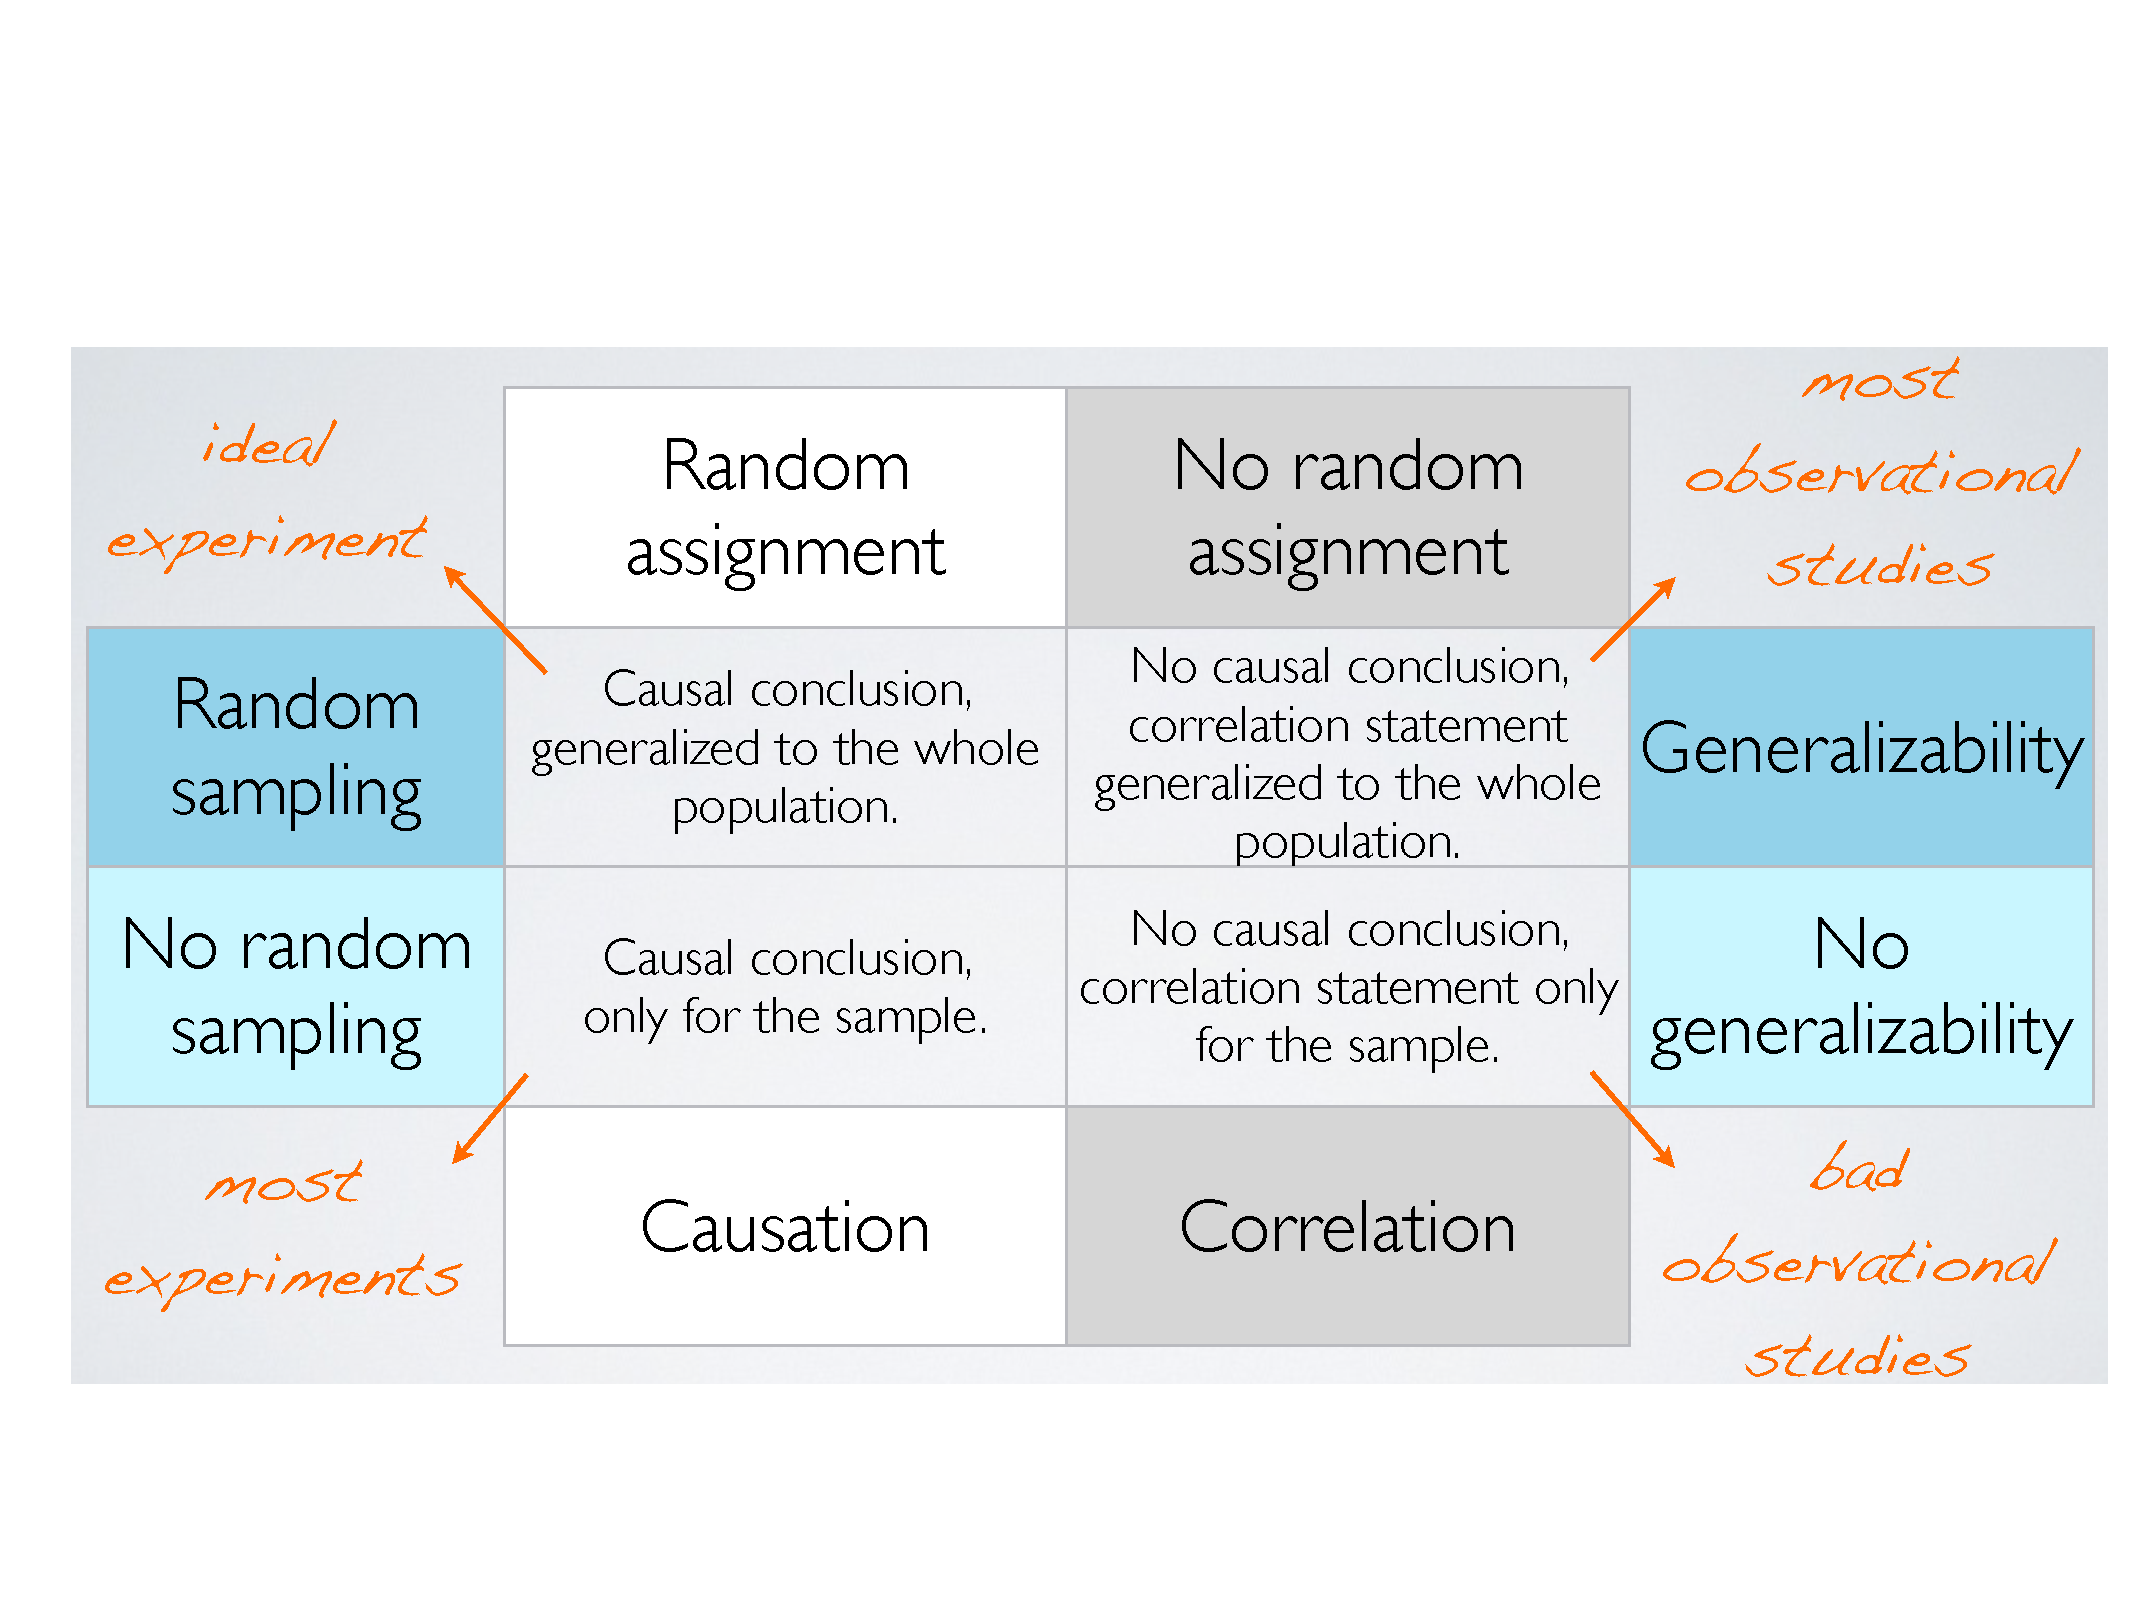
\includegraphics[width=\textwidth]{figures/random_sample_assignment}
\end{center}

\end{frame}

%%%%%%%%%%%%%%%%%%%%%%%%%%%%%%%%%%%

\section{Summary}

%%%%%%%%%%%%%%%%%%%%%%%%%%%%%%%%%%%

\begin{frame}
\frametitle{Summary of main ideas}

\vfill

\begin{enumerate}

\item \nameref{mi1}

\item \nameref{mi2}

\item \nameref{mi3}

\item \nameref{mi4}

\item \nameref{mi5}

\item \nameref{mi6}

\end{enumerate}

\vfill

\end{frame}

\end{document}